\chapter{Control Flow Graph construction}
\ref{chap:CFGConstruction}

\section{CFG construction for For and While loops}
\ref{sec:CFGConstructionLoops}
In this section we give examples of how we inductively generate the control flow graph of some essential language features. During this we will present the control flow graph nodes that we use, together with their semantics. \\
In Python, both for and while loops has an else branch, which is executed if the loop terminates normally (i.e. not using \inlinecode{break}).

\begin{listing}[H]
	\begin{minted}[linenos]{python}
"for" target_list "in" expression_list ":" suite 
["else" ":" suite]
	\end{minted}
	\caption{For-loop syntax according to the Python Language Reference}\label{code:forSyntax}
\end{listing}

\begin{listing}[H]
	\begin{minted}[linenos]{python}
for x in [1,2,3]:
  print x
else:
  print "not a break'ed exit"
	\end{minted}
	\caption{For-loop example}\label{code:forExample}
\end{listing}

\begin{wrapfigure}{r}{0.5\textwidth}
	\vspace{-20pt}
	\begin{center}
		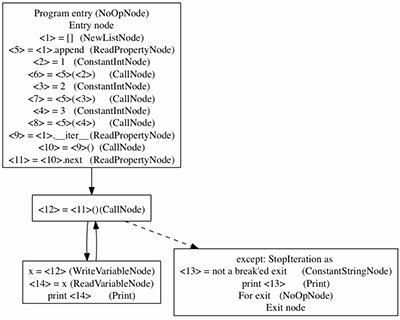
\includegraphics[width=0.48\textwidth]{images/for-example-cfg.png}
	\end{center}
	\vspace{-10pt}
	\caption{Control Flow Graph for the for-loop example \ref{code:forExample}}
	\label{fig:forCfg}
	\vspace{-10pt}
\end{wrapfigure}

First, \inlinecode{expression\_list} is evaluated. This should yield an iterable object, such that an iterator object can be created. Now for each element of the iterator the body of the for loop is evaluated once. As mentioned, if an else block is provided to the loop, it is evaluated when all iterations are done, and the iteration did not stop because of a break statement. \\
To simulate the evaluation sequence of such a for loop in our control flow graph, we need to take a look at the iterator object: to get the next element from a Python iterator object the next method is used. This method returns the next element until the iteration is done and finally raises a \inlinecode{StopIteration} exception. The CFG for the for-loop example \ref{code:forExample} can been seen in figure \ref{fig:forCfg}.

\begin{wrapfigure}{r}{0.5\textwidth}
	\vspace{-20pt}
	\begin{center}
		\includegraphics[width=0.48\textwidth]{images/while.png}
	\end{center}
	\vspace{-10pt}
	\caption{Control Flow Graph for a while-loop}
	\label{fig:whileCfg}
	\vspace{-10pt}
\end{wrapfigure}
For a while loop we generate the control flow graph in figure \ref{fig:whileCfg}.

\section{CFG cunstruction of With statements}
With statements in Python are unlike With statements in JavaScript.\ They are usually used when you have object you need to "open" before you do some work and then "close" it in the end, this pattern is used alot when working with I/O such as files or databases.\ An example of with statements can be seen in Listing \ref{code:withExample}.

\begin{listing}[H]
	\begin{minted}[linenos]{python}
with open('file.txt') as fh:
	print fh.read()
	\end{minted}
	\caption{With example reading a file}\label{code:withExample}
\end{listing}

The formal description of the With statement can be found in The Python Language Reference compound statement list\cite{pyref.compound} section 7.5, the hightlights is that if there is an \inlinecode{as} part of your with statement the result of the method call to \inlinecode{\_\_enter\_\_} assigned to the variable in the with statement. If there is raised an exception during the execution of the body of the With statement it is passed as arguments to the method call \inlinecode{\_\_exit\_\_}, if the result of that call returns something which truth value is \inlinecode{True} the with statement just evaluates normally, If a truth value of \inlinecode{False} is returned the exception isn't caught. If no exceptions happens during execution the \inlinecode{\_\_exit\_\_} method is called, after the body of the With statement, where \inlinecode{None} is passed as arguments.

\section{CFG construction of function and method calls}
\textit{CFG$_{\textit{cond}}$} is the control flow graph that results from the condition. If the condition is the boolean \inlinecode{True}, \textit{CFG$_{\textit{cond}}$} will be the control flow graph consisting of a single node, namely \textit{ConstantBooleanNode}. Inspired from TAJS, Type Analyzer for JavaScript, our \textit{ConstantBooleanNode} holds a result register (\textit{reg$_{\textit{cond}}$} in figure \ref{fig:callCfg}) together with the actual constant value, \inlinecode{True} in this case. \\
The other nodes \textit{ConstantIntNode}, \textit{ConstantFloatNode}, \textit{ConstantLongNode}, \textit{ConstantComplexNode}, \textit{ConstantStringNode}, \textit{ConstantNoneNode}, \textit{NewListNode}, \textit{NewDictionaryNode} and \textit{NewTupleNode} work in a similar way to \textit{ConstantBooleanNode}. \\
The motivation for introducing registers is that a single expression as e.g. \inlinecode{s1.addGrade('math', 10)} is evaluated in several steps. \\
First the function \inlinecode{addGrade} is looked up in the class of \inlinecode{s1}. This is done in the control flow graph using \textit{ReadPropertyNode}, which holds a result register, a base register, i.e. the register where to find the object, and the name of the property to look up. Similar nodes include \textit{ReadVariableNode} and \textit{ReadIndexableNode}. \\
\begin{wrapfigure}{r}{0.5\textwidth}
	\vspace{-20pt}
	\begin{center}
		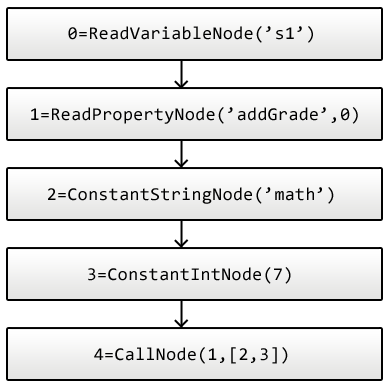
\includegraphics[width=0.48\textwidth]{images/Call-example.png}
	\end{center}
	\vspace{-10pt}
	\caption{Control Flow Graph for a call example}
	\label{fig:callCfg}
	\vspace{-10pt}
\end{wrapfigure}
Secondly, each argument given to the function is evaluated, and finally the actual call is done. Calls in the control flow graph is modeled using the \textit{CallNode}, which holds a result register, a function register and a list of arguments registers. \\
Thus the expression \inlinecode{s1.addGrade('math', 10)} will result in the control flow graph found in figure \ref{fig:callCfg} (where the numbers to the left represent the result registers of the nodes).\\
\todo{Tilfoeje afsnit om \_\_getattribute\_\_ og \_\_getattr\_\_, samt hvordan disse haandteres.} \\
So far we have primarily been concerned with putting constants into registers and reading e.g. variables. In order to support writing we have three different nodes: \textit{WriteVariableNode}, \textit{WritePropertyNode}, and \textit{WriteIndexableNode}. Besides holding a value register, i.e. the register where to find the value being written, \textit{WriteVariableNode} contains the name of the variable being written to, \textit{WritePropertyNode} contains a base register and the property being written to, and \textit{WriteIndexableNode} contains a base and property register (the latter has a register for the property because it is not constant, for instance we could write something like the following: \inlinecode{dict[getKey()] = aValue}, whereas property in \inlinecode{obj.property = aValue} must be a string).

\section{Handling exceptions}
In order to handle the flow caused by exceptions we use two different kinds of edges in the control flow graph. A solid edge indicates normal flow, and a dashed edge indicates exception flow. \\
In Python exceptions can be caught using a try-except-else-finally block. An except block can be annotated with a number of types, and each try-except-else-finally block may contain an arbitrary number of except blocks. As usual, the else block is entered in case of a normal exit, i.e. when no exceptions were raised inside the try block. \\
The AST provided by the Jython parser has been normalized from a try-except-else-finally block into a try-finally block, which contains a try-except-else block in its try block. \\
For instance the code in the first example \ref{code:tryExceptBefore} below is transformed into the code in the next example \ref{code:tryExceptAfter}:

\begin{listing}[H]
	\begin{minted}[linenos]{python}
try:
  <try-stms>
except Foo:
  <except-foo-stms>
except:
  <except-stms>
else: 
  <else>
finally:
  <finally>
	\end{minted}
	\caption{A try-except-else-finally example before convertion}\label{code:tryExceptBefore}
\end{listing}

\begin{listing}[H]
	\begin{minted}[linenos]{python}
try: 
  try:
    <try-stms>
  except Foo:
    <except-foo-stms>
  except:
    <except-stms>
  else:
    <else-stms>
finally:
  <finally-stms>
	\end{minted}
	\caption{A try-except-else-finally example after convertion}\label{code:tryExceptAfter}
\end{listing}

Inductively, CFG's for the statement lists <\inlinecode{try-stms}> (\textit{CFG$_{\textit{try}}$}), <\inlinecode{except-foo-stms}> (\textit{CFG$_{\textit{except-foo}}$}), <\inlinecode{except-stms}> (\textit{CFG$_{\textit{except}}$}), <\inlinecode{else-stms}> (\textit{CFG$_{\textit{else}}$}), and <\inlinecode{finally-stms}> are created. \\
The CFG for the finally block is then cloned into three duplicates (\textit{CFG$_{\textit{finally-normal}}$}, \textit{CFG$_{\textit{finally-handled-exc}}$}, \textit{CFG$_{\textit{finally-unhandled-exc}}$}). The purpose is to have one finally block for each of the following cases: 

\begin{enumerate}
  \item when no exceptions occur during the try block,
  \item when an exception is raised and caught by one of the surrounding except blocks, and no exception is raised from inside that except block, and
  \item when an exception is raised but not caught, which is the case when a) an exception is raised from
the try block and no except blocks handles this particular exception, b) an except block catches an exception raised by the try block, but then raises a new exception on its own.
\end{enumerate}

In particular, it is important that the finally block for handling case (3), i.e. \textit{CFG$_{\textit{finally-unhandled-exc}}$}, is not connected to the exit node of the try-except-else-finally block. Instead, it should be connected to its nearest surrounding except block (if any), or no except block at all (indicating that the program crashes with a runtime error because of an unhandled exception). \\
In the following sections we present the way we generate the CFG of a try-except-else-finally block.

\subsection{The try block}
Each node in \textit{CFG$_{\textit{try}}$} (that does not already have an outgoing exception edge) is connected using an exception edge to the entry node of the first except block (*), in this case the entry node of \textit{CFG$_{\textit{except-foo}}$}. We do not add exception edges to nodes that already have an exception edges, because this would be a loss of information: the control flow always goes to the nearest enclosing except block in case of exceptions. \\
The above models that if an exception occurs during evaluation of one of the statements in a try block, then the control flow will proceed from the first except block. \\
If there is no except blocks, each node should instead be connected using an exception edge to the entry node of its nearest surrounding except or finally block (specifially \textit{CFG$_{\textit{finally-unhandled-exc}}$}). However, we don't add any exception edges here; these will be added inductively because of (*) in case there are any surrounding except or finally blocks.

\begin{wrapfigure}{r}{0.5\textwidth}
	\vspace{-20pt}
	\begin{center}
		\includegraphics[width=0.48\textwidth]{images/Try-except-else-finally.png}
	\end{center}
	\vspace{-10pt}
	\caption{Control Flow Graph for try try-except example \ref{code:tryExceptAfter}}
	\label{fig:tryExceptCfg}
	\vspace{-10pt}
\end{wrapfigure}
\subsection{The except block}
The entry node of each except block is connected using an exception edge to the entry node of the next except block (except for the last block, of course). Thus we make an exception edge from the entry node of \textit{CFG$_{\textit{except-foo}}$} to the entry node of \textit{CFG$_{\textit{except}}$}. \\
We do this because the first except block might not catch the exception (because of the type restrictions), in which the control flow proceeds at the next except block. \\
Furthermore, each node inside the except block should be connected using an exception edge to the entry node of its nearest surrounding except or finally block (specifically \textit{CFG$_{\textit{finally-unhandled-exc}}$}). As above, this is handled inductively. \\
Finally, if an except block actually catches the exception, and no exceptions occur inside that except block, the control flow proceeds to the surrounding finally block (in this case, \textit{CFG$_{\textit{finally-handled-exc}}$}). 

\subsection{The else block}
If no exceptions occur, the else block should be evaluated. Thus we add a normal flow edge from the exit node of \textit{CFG$_{\textit{try}}$} to the entry node of \textit{CFG$_{\textit{else}}$}.\\
Since exceptions may result from evaluating the statements in the else block, each node in \textit{CFG$_{\textit{else}}$} should also be connected to the entry node of the nearest surrounding except or finally block (again, \textit{CFG$_{\textit{finally-unhandled-exc}}$}). \\
In case the evaluation of the statements in the else block does not raise any exceptions, the control flow proceeds either to the exit node of the whole try-except-else block, or in case there is a surrounding finally block, to the entry node of \textit{CFG$_{\textit{finally-normal}}$}.